\documentclass{article}
\usepackage{float}
\usepackage{graphicx}
%\usepackage{lipsum}
%\usepackage[margin=1in,includefoot]{geometry}

\begin{document}
\begin{titlepage}
	\begin{center}
	\line(1,0){300}\\
	[0.25in]
	\huge{\bfseries Literature Review: An investigation into the usefulness of Android Wear (Smart Watch)}\\
	[2mm]
	\line(1,0){200}\\
		\begin{figure}[H]
		\centering
		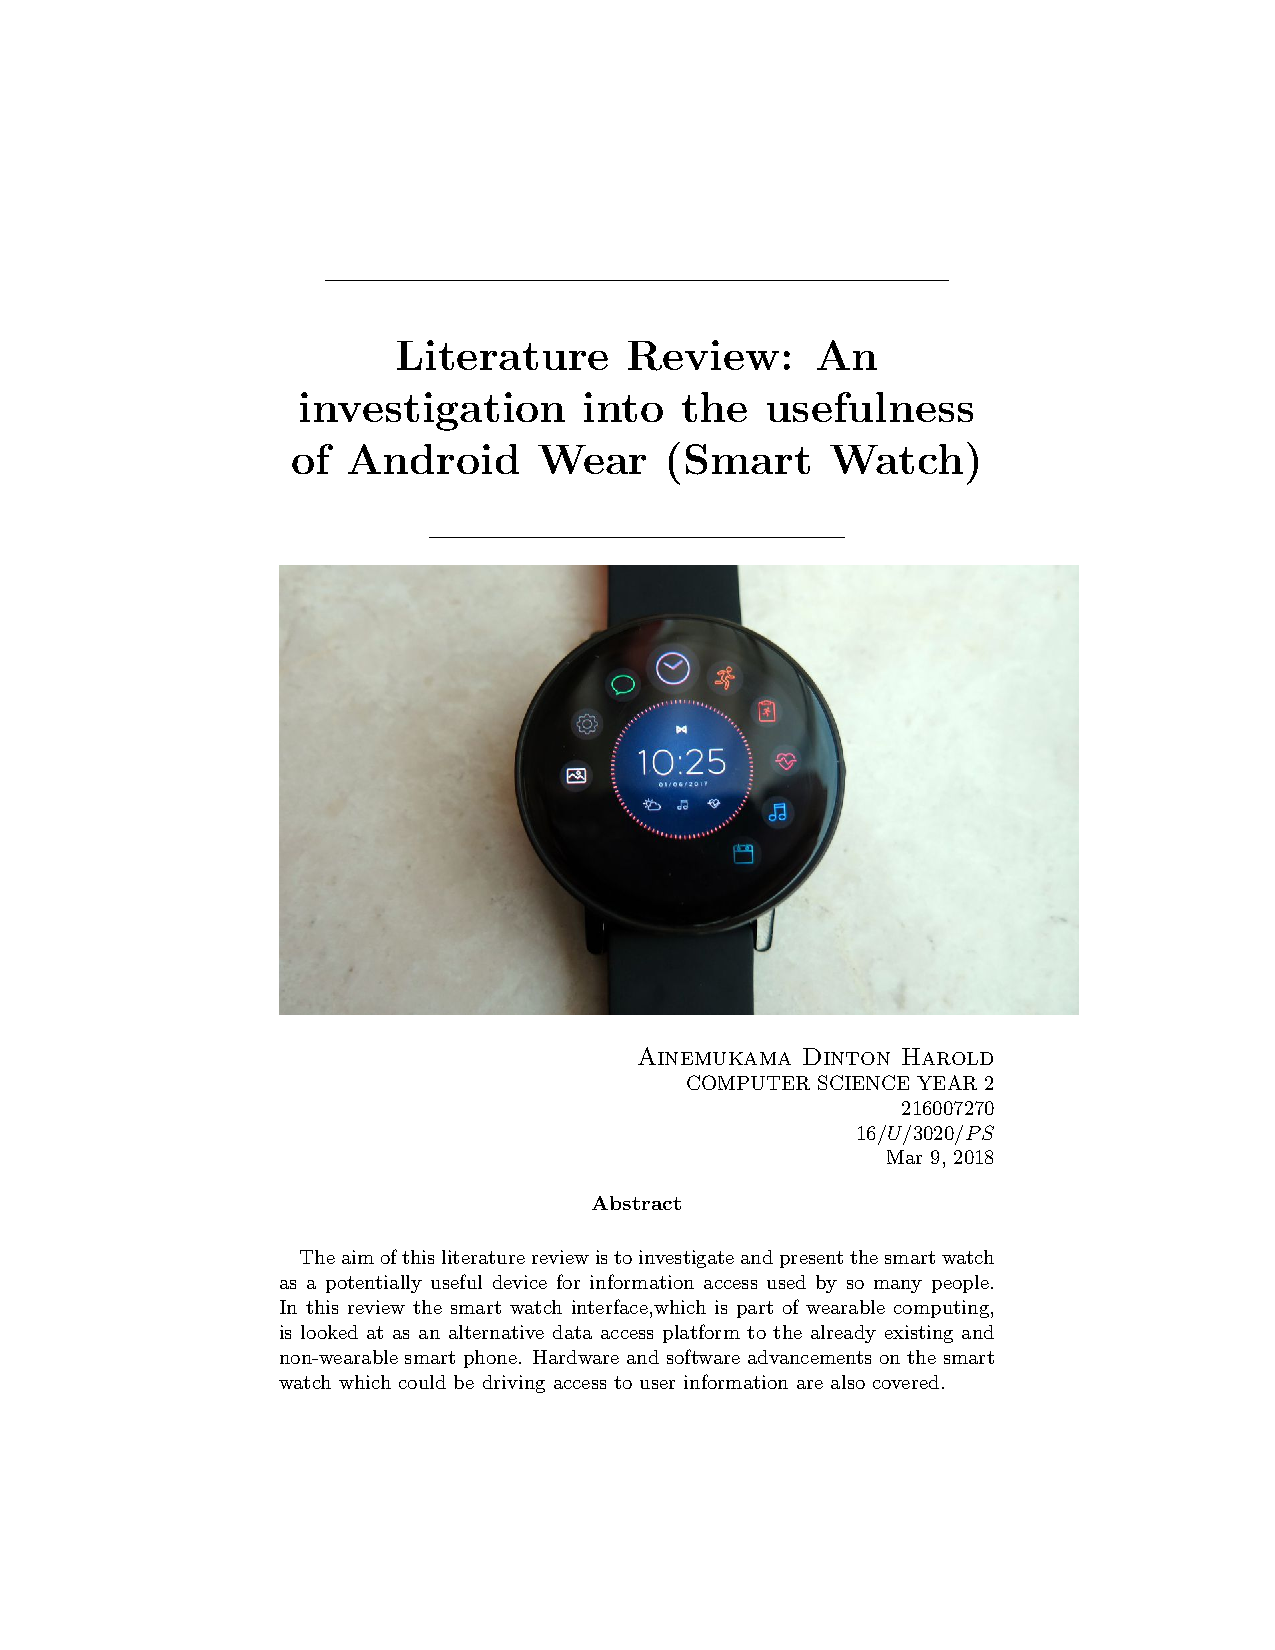
\includegraphics[height=3in]{/Users/Dintaine/Desktop/latex/figures/android.jpg}
		
		\end{figure}
	\end{center}
\begin{flushright}
\textsc{\large Ainemukama Dinton Harold}
 
 COMPUTER SCIENCE YEAR $2$\\
 $216007270$\\ 
 $16/U/3020/PS$\\
Mar 9, 2018\\
\end{flushright}
\begin{center}
{\bfseries Abstract}\\
\end{center}
\paragraph{}
The aim of this literature review is to investigate and present the smart watch as a potentially useful device for information access used by so many people. In this review the smart watch interface,which is part of wearable computing, is looked at as an alternative data access platform to the already existing and non-wearable smart phone. Hardware and software advancements on the smart watch which could be driving access to user information are also covered.
	
\end{titlepage}
\tableofcontents
\thispagestyle{empty}
\cleardoublepage

\setcounter{page}{1}
\section{Introduction}
With the introduction of the smart watch interface to the family of wearable computing devices,the question has been posed as to whether smart watches can provide their users with useful applications.Smart watches which were previously available on the market offered a limited number of applications at the discretion of manufacturers, with no intention of taking advantage of any open source software solutions\cite{r3}. The standardization of Application Programming Interfaces (API's) and the increasing availability of libraries through Software Development Kits(SDK's) for these devices, means that new applications can be created relatively quickly by developers and are able to meet the needs of users more dynamically than in the past\cite{r2}.
\section{The Smart Watch}
Using Rhodes definition\cite{r4} of wearable device requirements, it can be seen that the smart
watch meets these characteristics. The smart watch is: a) portable while still being accessible from the user's arm, b) allows for hands free operation, c) integrates sensors as input devices, d) communicates information to the user despite not being actively instructed to do so and e)continuously receives information on the surrounding environment.Marks\cite{r1} found that smart watches provided these attributes to their users by being an accessible and convenient method for accessing information;thus smart watches meet the requirements for wearable computing devices. In this section I will discuss the advantages and disadvantages of the smart watch.
\subsection{Advantages}\cite{r5}
Strong manufacturer and developer support.\\
Google Now cards and Knowledge Graph integration.\\
Hands-free voice control and Google voice search. 
\subsection{Disadvantages}\cite{r5}
Short battery life on current hardware.\\
Excessive notifications.\\
Only compartible with newer android devices.
\section{Summary}
Android Wear is the strongest smartwatch plaform we've seen so far, and it has enough support from manufactures and developers to thrive. But it's a first-generation product, and limited battery life, notification anxiety and other issues make it tough to recommend Wear quite just yet.
\bibliographystyle{IEEEtran}
\bibliography{references}

\end{document}
